\documentclass[../main.tex]{subfiles}

\begin{document}
\chapter{Konstruktion der Reellen Zahlen}
\section{Historische Motivation}
In der Antike war Mathematik praktisch synonym mit Geometrie. Der Zahlenbegriff war
direkt an das Konzept der \emph{Länge} gekoppelt.

\begin{definition}[Euklid, 300 vor Christus]
  Zwei Längen $a,b > 0$ heissen \emph{kommensurabel}, falls eine Länge $L>0$ existiert,
  so wie zwei natürliche Zahlen $m,n \in \mathbb N$, so dass $a = mL$ und $b=nL$.
\end{definition}

Hier ist
\[\mathbb N = \{0, 1, 2, 3, 4, \dots\}\]
die Menge der Natürlichen Zahlen.

\begin{theorem*}[Euklid]
  Die Seite und Diagonale eines ebenen Quadrats sind nicht kommensurabel.
\end{theorem*}

\begin{proof}
  Dieser Beweis ist geometrisch, nach Euklid. Wir nehmen an, es gäbe $L > 0$ und
  $m,n \in \mathbb N$ mit $x = mL$ und $d = nL$. Wir zeigen, dass das zu einem Widerspruch
  führt.
  Wir stellen fest, dass die Längen $x_{1} = d-x$ und $d_{1} = 2x - d$
  ebenfalls die Seite und Diagonale eines Quadrats bilden, siehe
  Abbildung~\ref{fig:euklid}.

  \begin{figure}[htb]
    \centering
    \begin{minipage}{0.4\linewidth}
      \centering
      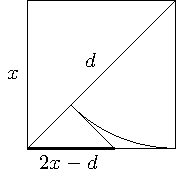
\includegraphics{images/euklid-quadrat}
    \end{minipage}%
    \begin{minipage}{0.4\linewidth}
      \centering
      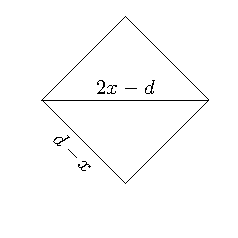
\includegraphics{images/euklid-quadrat2}
    \end{minipage}
    \caption{Euklids Konstruktion}%
    \label{fig:euklid}
  \end{figure}

  Weiterhin gilt, dass sowohl $x_{1}$ als auch $d_{1}$, ganze Vielfache von $L$ sind:
  \begin{align*}
    x_{1} = d-x = (n-m)L \\
    d_{1} = 2x-d = (2m -n)L
  \end{align*}
  Nach Pythagoras gilt $d^{2} = 2x^{2}$, und somit $d \leq 3/2\cdot x$, da ${(3/2)}^{2} > 2$.
  Daraus folgt, dass
  \[x_{1} = d - x \leq \frac{1}{2} \cdot x.\]
  Iteriere dieses Verfahren und erhalte eine Serie von Quadraten mit Seiten
  $x_{2}, x_{3}, \dots$ und Diagonalen $d_{2}, d_{3}, \dots$. Es gilt:
  \[x_{k} \leq \frac{1}{2^{k}} \cdot x.\]
  Ausserdem ist jedes $x_{k}$ (und $d_{k}$) ein ganzes Vielfaches von $L$.
  Wähle nun $k$ so gross, dass
   \[x_{k} \leq \frac{1}{2^{k}} x < L.\]

   Dies, zusammen mit dem Fakt, dass
   $x_{k}$ ein ganzes Vielfaches von $L$ ist,
   impliziert, dass $x_{k} = 0$, was unmöglich ist. Deshalb können $x$ und $d$
   nicht kommensurabel sein.
\end{proof}

Wir haben diese Aussage mit einem sogenannten \emph{Widerspruchsbeweis} bewiesen.
Hierfür haben wir eine Annahme getroffen, und diese zu einem Widerspruch geführt.
Dies zeigt, dass unsere Annahme falsch war.

\subsection*{Zeitgenössische Umformulierung}
Seien $a,b > 0$ zwei kommensurable Längen. Das heisst, es existieren $L > 0$
und $m,n \in \mathbb N$ mit $a = mL$, $b= nL$. Dann gilt:
\[\frac{a}{b} = \frac{mL}{nL} = \frac{m}{n},\]
das heisst das Verhältnis $a/b$ ist eine \emph{rationale Zahl}.
Zurück zum Quadrat mit Seite $x$ und Diagonale $d$. Nach Pythagoras
gilt $d^{2} = 2x^{2}$. Falls $x=mL$ und $d=nL$ gilt,
dann also
\[2 = \frac{d^{2}}{x^{2}} = {\left( \frac{d}{x}\right)}^{2} = {\left(\frac{n}{m}\right)}^{2},\]
und somit
\begin{equation}
  \label{eq:1}
2m^{2} = n^{2}.
\end{equation}
Die linke Seite dieser Gleichung ist durch $2$ teilbar. Dies impliziert, dass $n^{2}$, und
somit auch $n$, durch $2$ teilbar ist. Schreibe nun $n = 2k$. Schreibe $n = 2k$ mit
$k \in \mathbb N$. Setze das in die Gleichung~(\ref{eq:1}) ein und erhalte
$2m^{2} = {(2k)}^{2} = 4k^{2}$,
beziehungsweise
\[m^{2} = 2k^{2}.\]
Die rechte Seite ist durch $2$ teilbar, also auch $m$.
Wir schliessen, dass sowohl $n$ als auch $m$ durch $2$ teilbar sind.
Schreibe noch $m = 2\ell$ mit $\ell \in \mathbb N$. Es gilt also
\[ 2 = {\left(\frac{n}{m}\right)}^{2}
  = {\left(\frac{k}{\ell}\right)}^{2}.\]
In anderen Worten sind Zähler und Nenner beide gerade.
Iteriere dieses Verfahren $k$ mal, bis $n/2^{k} < 1$, Dann entsteht ein Widerspruch.

\begin{corollary}
  Die Gleichung $z^{2} = 2$ hat keine rationale Lösung, das heisst,
  keine Lösung der Form $z = p/q$ mit $p, q \in \mathbb N$ und $q > 0$.
\end{corollary}

Das Ziel für den Rest dieses Kapitels ist es, eine Zahlenmenge $\mathbb R$ (die Menge
der \emph{reellen Zahlen}) zu konstruieren, in welcher die Gleichung
$z^{2} = 2$ eine Lösung hat.

\begin{exercise}
  Die Gleichung $z = \sqrt 2 x + \sqrt 3 y$ hat keine ganze Lösungen ausser $(0,0,0)$.
\end{exercise}

\section{Mengen im Vergleich}
Wir haben bereits einige Mengen erwähnt, nämlich die \emph{natürlichen Zahlen}
\[ \mathbb N = \{0, 1, 2, 3, \dots\},\]
die Menge der \emph{ganzen Zahlen},
\[ \mathbb Z = \{0, 1, -1, 2, -2, \dots\},\]
und die Menge der \emph{rationalen Zahlen}
\[ \mathbb Q = \left\{p/q \mid p, q \in \mathbb Z, \, q > 0\right\}.\]
Wir wollen eine weitere Menge, die Menge $\mathbb R$ der \emph{reellen Zahlen}
einführen. Es gelten dann die Inklusionen
\[\mathbb N \subset \mathbb Z \subset \mathbb Q \subset \mathbb R.\]

\subsection*{Wichtige Grundbegriffe}
\begin{definition}
  Seien $A, B$ zwei Mengen.
  Eine \emph{Abbildung} zwischen $A$ und $B$,
  in Symbolen, $f \colon A \to B$, ist eine Zuordnung
  $f(a) \in B$ für jedes $a \in A$.
  Eine Abbildung $f \colon A \to B$ heisst
  \begin{enumerate}[(i)]
    \item \emph{injektiv}, falls für alle $a_{2}, a_{1} \in A$
      mit $a_{2} \ne a_{1}$ gilt, dass $f(a_{1}) \neq f(a_{2})$,
    \item \emph{surjektiv}, falls für alle $b \in B$ ein Element
      $a \in A$ existiert mit $f(a) = b$,
      \item \emph{bijektiv}, falls $f$ sowohl injektiv als auch surjektiv ist.
  \end{enumerate}
\end{definition}

\begin{example}\label{ex:inj-surj}
  \leavevmode
  \begin{enumerate}[(i)]
    \item Seien $A = B = \{0, 1\}$. Es gibt $4$ Abbildungen $f \colon A \rightarrow B$:
      \begin{enumerate}[(a)]
        \item $0 \mapsto 0$ und $1 \mapsto 0$,
        \item $0 \mapsto 1$ und $1 \mapsto 1$,
        \item $0 \mapsto 0$ und $1 \mapsto 1$,
        \item $0 \mapsto 1$ und $1 \mapsto 0$.
      \end{enumerate}
      Abbildungen (a) und (b) sind weder injektiv noch surjektiv. Abbildungen (c) und (d) sind
      beide bijektiv.
    \item Seien $A = B = \mathbb N$. Betrachte die Abbildung
      \begin{align*}
        f \colon \mathbb N &\to \mathbb N \\
        n &\mapsto 2n.
      \end{align*}
      Diese Abbildung ist injektiv, aber nicht surjektiv. Die Abbildung
      \begin{align*}
        g \colon \mathbb N &\to \mathbb N \\
            n &\mapsto \frac{2n - 1 + {(-1)}^{n}}{4},
      \end{align*}
      also die Abbildung die durch $2$ dividiert und dann abrundet, ist nicht injektiv,
      aber surjektiv. Um zu sehen, dass
      $g(n) = \lfloor{n/2}\rfloor$, betrachte zwei Fälle:
      \begin{enumerate}[(a)]
        \item $n = 2k$ ist gerade. Dann ist $g(n) = (4k+1-1)/4 = k$.
        \item $n = 2k + 1$ ist ungerade. Dann ist $g(n) = (4k + 2 -1 -1)/4 = k$.
      \end{enumerate}
  \end{enumerate}
\end{example}

\begin{remark}
  \leavevmode
  \begin{enumerate}[(1)]
    \item Bijektive Abbildungen $f \colon A \to B$ haben eine eindeutige \emph{Umkehrabbildung}
      $f^{-1} \colon B \to A$. Die Konstruktion dafür ist wie folgt. Sei $b \in B$.
      Da $f$ surjektiv ist, existiert $a \in A$ mit $f(a) = b$. Da $f$
      injektiv ist, ist dieses $a$ eindeutig. Setze $f^{-1}(b) = a$. Es gilt dann
      \[f^{-1}(f(a)) = a\]
      für alle $a \in A$, und ebenso
      \[f(f^{-1}(b)) = b\]
      für alle $b \in B$. Wir schreiben häufig
      \begin{align*}
        f^{-1} \circ f = \textrm{Id}_{A}, \\
        f \circ f^{-1} = \textrm{Id}_{B},
      \end{align*}
      in Worten, ``$f^{-1}$ verknüpft mit $f$ ist die Identitätsabbildung auf $A$''
      und ähnlich, ``$f$ verknüpft mit $f^{-1}$ ist die Identitätsabbildung auf $B$''.
    \item Für endliche Mengen $A$ und $B$ gilt: Es existiert eine bijektive Abbildung
      $f: A \to B$, genau dann, wenn $A$ und $B$ gleich viele Elemente haben.
  \end{enumerate}
\end{remark}

\begin{definition}
  Eine Menge $A$ heisst
  \begin{enumerate}[(i)]
    \item \emph{unendlich}, falls eine injektive, nicht surjektive Abbildung
      $f: A \to A$ existiert,
    \item \emph{abzählbar}, falls eine bijektive Abbildung $f \colon \mathbb N \to A$
      existiert.
  \end{enumerate}
\end{definition}

\begin{example}
  Sei $A = \mathbb N$. Die Abbildung $f$ aus Beispiel~(ii) ist injektiv,
  aber nicht surjektiv. Also ist $\mathbb N$ eine unendliche Menge.
\end{example}

\begin{example}
  Sei $M$ eine Menge, welche $\mathbb N$ als Teilmenge enthält
  (zum Beispiel $M = \mathbb Q$).
  Dann ist $M$ unendlich. Betrachte dazu die Abbildung
  \begin{align*}
    f \colon M &\to M \\
    x &\mapsto
      \begin{cases}
        x+1 & \mbox{falls }x \in \mathbb N \subset M, \\
        x & \mbox{falls }x \in M \setminus \mathbb N
      \end{cases}
  \end{align*}
\end{example}

Folgende Proposition zeigt in einem gewissen Sinn, dass es gleich viele Brüche
wie natürliche Zahlen gibt. Dies ist unser erstes potentiell überraschendes
Resultat.

\begin{proposition}\label{prop:q-countable}
  Die Menge $\mathbb Q$ der rationalen Zahlen ist abzählbar.
\end{proposition}


\begin{proof}
  Wir konstruieren eine Bijektion $\varphi \colon \mathbb N \to \mathbb Q$.
  Für $k \in \mathbb N$ mit $k \geq 1$ definiere
  \[
    A_{k} = \left\{p/q \mid p, q \in \mathbb Z, q \geq 1, p/q \textup{ ist gekürzt},
    |p| + |q| = k\right\}.
  \]
  Alle solchen $A_{k} \subset \mathbb Q$ sind endlich und
  \[
    \mathbb Q = \bigcupdot_{k \geq 1} A_{k}
  \]
  ist die \emph{disjunkte Vereinigung} dieser Mengen.
  Wir haben
  \[
    A_{1} = \{0/1\}, \; A_{2} = \{\pm 1/1\}, \; A_{3} = \{\pm 1/2, \pm 2/1\}, \dots.
  \]
  Sei $a_{k} = |A_{k}|$ die Anzahl Elemente von $A_{k}$.
  Definiere Teilmengen $B_{k} \subset \mathbb N$ mit $|B_{k}| = a_{k}$.
  Dazu setze $B_{1} = \{0\}$, und für $k \geq 2$ setze
  \[
    B_{k} = \{a_{1} + \cdots + a_{k-1},
    a_{1} + \cdots + a_{k-1} + 1, \dots,
    a_{1} + \cdots + a_{k-1} + a_{k} - 1\}.
  \]
  Es gilt dann
  \[
    B_{1} = \{0\}, \; B_{2} = \{1, 2\}, \; B_{3} = \{3, 4, 5, 6\}, \dots.
  \]
Wähle eine Bijektion $\varphi_{k} \colon B_{k} \to A_{k}$ für alle $k \geq 1$.
Definiere nun
\begin{align*}
  \varphi \colon \mathbb N &\to \mathbb Q \\
  n &\mapsto \varphi_{k}(n) \;\text{falls}\; n \in B_{k}.
\end{align*}
Die Abbildung $\varphi$ ist eine Bijektion, da $\mathbb N$ die disjunkte
Vereinigung der $B_{k}$ und $\mathbb Q$ die disjunkte Vereinigung
der $A_{k}$ ist.
\end{proof}

Dieser Beweis zeigt allgemeiner, dass jede Menge, die eine abzählbare Vereinigung
endlicher Mengen ist, selber abzählbar ist. Man könnte diese Aussage
zum Beispiel für Aufgabe 5 auf Serie 1 verwenden.

\begin{question}
  Ist jede unendliche Menge abzählbar?
\end{question}

Georg Cantor hat ca. 1870 als erste Person die Antwort ``nein'' auf diese Frage
festgehalten.
Wir konstruieren nun nach seiner Idee
eine Menge, die nicht abzählbar ist.
Dazu betrachten wir die \emph{Potenzmenge} $P(M)$
einer Menge $M$, definiert als die ``Menge aller Teilmengen von $M$''.
Ein wenig formaler,
\[P(M) = \left\{A \mid A \subset M\right\}.\]

\begin{example}
  Sei $M = \{0, 1\}$. Dann ist
  \[
    P(M) = \{ \emptyset, \{0\}, \{1\}, \{0, 1\}\}.
  \]
  Das Symbol $\emptyset$ bezeichnet die \emph{leere Menge}.
\end{example}

\begin{remark}
  Falls die Menge $M$ selbst $n$ Elemente hat, dann hat ihre
  Potenzmenge $2^{n}$ Elemente. Um das zu beweisen,
  bilden wir jede Teilmenge $A$ von $M$
  auf die Funktion
  \begin{align*}
    f_{A} \colon  M &\to \{0, 1\} \\
     x &\mapsto
      \begin{cases}
        0, & \mbox{falls } x \notin A, \\
        1, & \mbox{falls } x \in A,
      \end{cases}
  \end{align*}
  ab.
  Diese Abbildung $A \mapsto f_{A}$ ist eine Bijektion zwischen
  $P(M)$ und der Menge von Funktionen $f \colon M \to \{0, 1\}$,
  und es gibt $2^{n}$
  solche Funktionen.
\end{remark}

\begin{proposition}[Cantor]\label{prop:cantor}
  Sei $M$ eine beliebige Menge.
  Dann existiert keine surjektive Abbildung $\varphi \colon M \to P(M)$.
  Insbesondere existiert keine Bijektion $\varphi \colon M \to P(M)$.
\end{proposition}

\begin{corollary}
  Die Potenzmenge $P(\mathbb N)$ ist nicht abzählbar.
\end{corollary}

\begin{proof}[Beweis der Proposition]
  Wir führen einen klassischen Widerspruchsbeweis.
  Wir nehmen an, es gäbe doch eine solche Surjektion
  $\varphi \colon M \to P(M)$.
  Betrachte nun die Teilmenge $A$ von $M$ aller $x$, die nicht
  in $\varphi(x)$ enthalten sind. In Symbolen,
  \[
    A = \left\{x \in M \mid x \notin \varphi(x)\right\}.
  \]
  Die Forderung $x \notin \varphi(x)$ macht Sinn,
  da $\varphi(x)$ selbst eine Teilmenge von $M$ ist.
  Da $\varphi$ surjektiv ist, muss ein $a \in M$
  existieren mit $\varphi(a) = A$. Wir fragen nun,
  ob $a \in A$ ist oder nicht.
  Wäre $a \in A$, so müsste nach Definition von $A$
  gelten, dass $a \notin \varphi(a)$. Aber das
  widerspricht der Definition von $\varphi(a) = A$.
  Wäre jedoch $a \notin A$, dann wäre die Bedingung
  $a \notin \varphi(a)$ erfüllt, also $a \in A$.
  Aber da $A = \varphi(a)$, widerspricht auch dies
  der Definition von $A$. Somit führen beide Möglichkeiten
  zu einem Widerspruch. Dies bedeutet, dass unsere
  ursprüngliche Annahme, dass eine Surjektion
  $\varphi \colon M \to P(M)$ existiert, verworfen werden muss:
  Es kann keine solche Abbildung geben.
\end{proof}

\subsection*{Einschub: Beweismethoden}
Ein \emph{Beweis} ist eine ``Deduktion einer Aussage
aus bereits bewiesenen Aussagen oder Grundaxiomen''.
Wichtig ist hier, dass die Deduktion logisch korrekt erfolgt.
Folgende Beweismethoden sind typisch.
  \begin{itemize}
    \item Geometrische Beweise, zum Beispiel mit Hilfe von Euklids Axiomen.
      Das erste Theorem der Vorlesung haben wir so bewiesen.
    \item Beweise mithilfe von logischen Schlussfolgerungen,
      zum Beispiel Widerspruchsbeweise.
      Proposition~\ref{prop:cantor} haben wir so bewiesen.
    \item Kombinatorische Beweise, zum Beispiel
      Beweise mit vollständiger Induktion.
  \end{itemize}


Wir führen nun ein Beispiel eines Beweises durch vollständige Induktion.
\begin{definition}
  Die $n$-te \emph{Catalanzahl} $C_{n}$ ist die Anzahl korrekte
  Klammerungen mit $2n$ Klammern ($n$ linke und $n$ rechte Klammern).
\end{definition}

\begin{examples}
  \leavevmode
  \begin{itemize}
    \item
        $C_{1} = 1$, die einzige Korrekte Klammerung ist $()$.
    \item
      $C_{2} = 2$, die Klammerungen $()()$ und $(())$ sind beide korrekt.
    \item $C_{3} = 5$.
  \end{itemize}
\end{examples}

\begin{claim}
  Die $n$-te Catalanzahl $C_{n}$ erfüllt $C_{n} \geq 2^{n-1}$.
\end{claim}

\begin{proof}[Beweis durch vollständige Induktion]
  Für die \emph{Induktionsverankerung} testen wir die Aussage für $n = 1$:
  Tatsächlich
  ist $C_{1} \geq 2^{0}$.

  Die \emph{Induktionsannahme} ist nun,
  dass die Aussage für ein festes $n \in \mathbb N$ stimmt.

  Im \emph{Induktionsschritt} leiten wir nun die Aussage für $n + 1$
  aus der Induktionsannahme (für $n$) her.
  Hier heisst das, dass wir $C_{n+1} \geq 2^{n}$ aus $C_{n} \geq 2^{n-1}$
  herleiten wollen. Sei dazu $K$ eine korrekte $n$-Klammerung,
  das heisst eine korrekte
  Klammerung mit $n$ linken und $n$ rechten Klammern.
  Dann sind sowohl $(K)$ als auch $()K$ korrekte $(n+1)$-Klammerungen.
  Weiter gilt, dass diese beiden Klammerungen verschieden sind:
  Die erste der beiden Klammerungen beginnt mit zwei geöffneten Klammern,
  wobei die zweite mit einer geöffneten und einer geschlossenen
  Klammer beginnt.
  Weiter gilt, dass für verschiedene
  korrekte $n$-Klammerungen $K_{1}$ und $K_{2}$
  auch $()K_{1}, (K_{1}), ()K_{2}, (K_{2})$ verschieden sind (wieso?).
  Wir können also aus jeder korrekten $n$-Klammerung zwei korrekte
  $(n+1)$-Klammerungen konstruieren. Somit folgt, dass
  \[C_{n+1} \geq 2 C_{n} \geq 2 \cdot 2^{n-1} = 2^{n}.\]
  Dies zeigt die Aussage für $n+ 1$.
\end{proof}

In Serie 1 sehen wir, dass sogar $C_{n} \geq 3^{n}$ gilt,
jedenfalls für $n \geq 17$.
Um dies zu zeigen reicht es aber nicht, zu bemerken,
dass neben $(K)$ und $()K$ auch $K()$ eine korrekte
Klammerung ist. Diese könnte nämlich mit $()K$
übereinstimmen.
Hierzu brauchen wir die Formel in folgender Bemerkung.

\begin{remark}
  Es gilt
  \[
    C_{n} = \binom{2n}{n} - \binom{2n}{n+1} = \frac{1}{n+1}\binom{2n}{n}.
  \]
  Die zweite Gleichheit ist eine einfache Rechnung.
  Wir rechtfertigen die erste Gleichheit.
  Der erste der Binomialkoeffizienten zählt alle $n$-Klammerungen (auch inkorrekte).
  Der zweite Binomialkoeffizient zählt die Anzahl inkorrekter Klammerungen.
  Man kann sich dies folgendermassen skizzenhaft überlegen.
  Eine inkorrekte Klammerung hat eine erste Position,
  wo eine rechte Klammer zuviel ist.
  Drehe alle Klammern hinter dieser Position um.
  Die Klammerung die wir so erhalten, hat $n+1$ rechte Klammern.
  Weiter kann man diesen Prozess rückgängig machen:
  Jede Klammerung mit $n+1$ rechten Klammern
  liefert eine inkorrekte Klammerung mit $n$ rechten Klammern.
  Also sind die schlechten $n$-Klammerungen in Bijektion
  mit der Anzahl Klammerungen mit $n+1$ rechten
  (und $n-1$ linken) Klammern.
\end{remark}

\section{Gruppen und Körper}
\begin{definition}
  Eine \emph{Gruppe} ist eine Menge $G$
  mit einer \emph{Verknüpfung} $\circ \colon G \times G \to G$,
  welche folgende Eigenschaften erfüllt.
  \begin{enumerate}[(i)]
    \item Es existiert ein Element $e \in G$, so dass
      für alle $g \in G$ gilt, dass
      $g \circ e = e \circ g = g$.
    \item Für alle $g \in G$ existiert ein $h \in G$
      mit
      $g \circ h = h \circ g = e$.
    \item Für alle $a,b,c \in G$ gilt
      $(a \circ b) \circ c = a \circ (b \circ c)$.
  \end{enumerate}
\end{definition}

\begin{notation}
  \leavevmode
  \begin{enumerate}[(i)]
    \item Das Element $e$ bezeichnen wir als das \emph{neutrale Element}.
    \item Wir schreiben häufig $g^{-1}$ für $h$ und nennen $g^{-1}$
      das zu $g$ \emph{inverse Element}.
    \item Das Gesetz $(a \circ b) \circ c = a \circ (b \circ c)$ nennt man das \emph{Assoziativgesetz}.
  \end{enumerate}
\end{notation}

\begin{examples}
  \leavevmode
  \begin{itemize}
    \item Die Menge $G = \{e\}$ mit der Operation
      $e \circ e = e$ ist eine Gruppe (sie heisst \emph{triviale Gruppe}).
    \item Die Menge $\{e, a\}$ mit Verknüpfungstabelle zu finden
      in Tabelle~\ref{tab:ea} bildet eine Gruppe.
      \begin{table}[htb]
        \centering
        \begin{tabular}[h]{ccc}
         & \color{gray}{$e$} & \color{gray}{$a$}\\
        % \hline
        \color{gray}{$e$} & $e$ & $a$ \\
        \color{gray}{$a$} & $a$ & $e$
        \end{tabular}
        \caption{Verknüpfungstabelle von $\{e, a\}$}%
        \label{tab:ea}
      \end{table}

    \item Die Menge $\{e, a, b\}$ mit Verknüpfungstabelle zu finden
      in Tabelle~\ref{tab:eab} bildet eine Gruppe.
      Hier kann man $a$ als ebene Drehung um $0$ mit Winkel $2\pi/3$
      interpretieren. Ähnlich ist $b$ eine Drehung mit
      Winkel $4\pi/3$.
      \begin{table}[htb]
        \centering
        \begin{tabular}[h]{cccc}
        & \color{gray}$e$ & \color{gray}$a$ & \color{gray}$b$\\
        % \hline
        \color{gray}$e$ & $e$ & $a$ & $b$\\
        \color{gray}$a$ & $a$ & $b$ & $e$ \\
        \color{gray}$b$ & $b$ & $e$ & $a$
        \end{tabular}
        \caption{Verknüpfungstabelle von $\{e, a, b\}$}%
        \label{tab:eab}
      \end{table}
      \item $(Z, +)$ ist eine Gruppe.
      \item $(\mathbb Z, \cdot)$ ist keine Gruppe. Zum Beispiel hat die Zahl
      $2 \in \mathbb Z$ kein inverses Element.
      \item $(\mathbb Q, +)$ ist eine Gruppe.
      \item $(\mathbb Q, \cdot)$ ist keine Gruppe. Zum Beispiel hat $0 \in \mathbb Q$
      kein inverses Element.
  \end{itemize}
\end{examples}

\begin{proposition}
  In jeder Gruppe $G$
  hat die Gleichung $a \circ x = c$
  eine eindeutige Lösung $x \in G$. Hier sind $a,c$ vorgegeben.
\end{proposition}

\begin{proof}
  Wir zeigen Existenz und Eindeutigkeit separat. Wir wissen nach
  Axiom~(ii), dass $b \in G$ existiert mit $b \circ a = e$.
  Verknüpfung mit $b$ von links auf beiden Seiten liefert
  $b \circ (a \circ x) = b \circ c$. Axiom~(iii) sagt, dass
  die linke Seite
  \[
    (b \circ a) \circ x = e \circ x = x
  \]
  ist. Also ist $x = b \circ c = a^{-1} \circ c$ eine Lösung.
  Um Eindeutigkeit zu zeigen seien $x_{1}, x_{2} \in G$ mit
  \[
    a \circ x_{1} = c = a \circ x_{2}.
  \]
  Verknüpfung von links wie oben mit $b$ liefert
  \[b \circ (a \circ x_{1}) = b \circ (a \circ x_{2}).\]
  Wir erhalten
  \[
    (b \circ a) \circ x_{1} = (b \circ a) \circ x_{2}.
  \]
  Sobald wir uns erinnern, dass $b \circ a = e$, schliessen wir,
  dass $x_{1} = x_{2}$.
\end{proof}

\begin{specialcases}
  \leavevmode
  \begin{enumerate}[(1)]
    \item Falls $a \circ x = a$ gilt, so ist $x = e$. Dies liefert Eindeutigkeit
      des neutralen Elements.
    \item Falls $a \circ x = e$ gilt, so ist $x = a^{-1}$. Dies liefert
      Eindeutigkeit des inversen Elements.
  \end{enumerate}
\end{specialcases}

\subsection*{Körper}
\begin{definition}
  Eine Menge $K$ mit zwei Verknüpfungen $+, \cdot \colon K \times K \to K$ heisst
  \emph{Körper}, falls
  \begin{enumerate}[(i)]
    \item $(K, +)$ ist eine kommutative Gruppe mit neutralem
      Element $0 \in K$,
    \item $(K \setminus \{0\}, \cdot)$ ist eine kommutative Gruppe
      mit neutralem Element $1 \in K \setminus \{0\}$ (das heisst $1 \neq 0$),
    \item für alle $x,y,z \in K$ gilt das
      Distributivgesetz $x \cdot (y + z) = x \cdot y + x \cdot z$.
  \end{enumerate}
\end{definition}

Wir halten uns hier an die Konvention, dass die Multiplikation stärker
bindet als die Addition. Konkret haben wir oben
\[ x \cdot y + x \cdot z = (x \cdot y) + (x \cdot z).\]
Dass $(G, \circ)$ eine kommutative Gruppe ist, bedeutet,
dass für alle $g, h \in G$ gilt, dass $g \circ h = h \circ g$.

\begin{examples}
  \leavevmode
  \begin{enumerate}[(1)]
    \item $K = \mathbb Q$ mit der üblichen Addition
      \[ \frac{a}{b} + \frac{c}{d} = \frac{ad + bc}{bd}\]
      und üblichen Multiplikation
      \[ \frac{a}{b} \cdot \frac{c}{d} = \frac{ac}{bd}\]
      bildet einen Körper mit neutralen Elementen $0/1$ (für $+$) und $1/1$ (für $\cdot$).
      Die Rechengesetze (Assoziativität, Kommutativität und Distributivität) übertragen
      sich von den entsprechenden Gesetzen für die Menge der ganzen Zahlen $\mathbb Z$
      mit der üblichen Addition und Multiplikation.
      Diese widerum wurden von Dedekind erstmals formal definiert (``was
      sind und sollen Zahlen'').
      % TODO
      Wir
      führen das in dieser Vorlesung nicht weiter aus.
    \item $K = \{0, 1\}$ mit Verknüpfungstabellen
      wie in Tabelle~\ref{tab:01}
      \begin{table}[h]
        \centering
        \begin{minipage}{0.25\linewidth}
          \centering
        \begin{tabular}[h]{ccc}
         $+$ & \color{gray}{$0$} & \color{gray}{$1$}\\
        % \hline
        \color{gray}{$0$} & $0$ & $1$ \\
        \color{gray}{$1$} & $1$ & $0$
        \end{tabular}%
        \end{minipage}%
        \begin{minipage}{0.25\linewidth}
          \centering
        \begin{tabular}[h]{ccc}
          $\cdot$ & \color{gray}{$0$} & \color{gray}{$1$} \\
          \color{gray}{$0$} & $0$ & $0$ \\
          \color{gray}{$1$} & $0$ & $1$
        \end{tabular}
      \end{minipage}
      \caption{Verknüpfungstabellen von $\{0, 1\}$}%
      \label{tab:01}
      \end{table}
      ist ein Körper (der kleinste).
    \item $(\mathbb Z, + , \cdot)$ ist kein Körper, da nur $\pm 1$ multiplikative
      Inverse haben.
  \end{enumerate}
\end{examples}

\begin{ausblick}[Algebra]
  Sei $p \in \mathbb N$ prim. Dann ist die Menge
  \[ \mathbb Z / p \mathbb Z = \{0, 1, 2, \dots, p-1\}\]
  mit ``Addieren und Multiplizieren modulo $p$'' ein Körper.
\end{ausblick}

\section{Konstruktion der reellen Zahlen}
\begin{goal}
  Wir konstruieren eine Zahlenmenge $\mathbb R$,
  die Menge der reellen Zahlen, mit folgender
  Eigenschaft: Jede stetige Funktion $f \colon \mathbb R \to \mathbb R$,
  welche negative und positive Werte annimmt, hat eine Nullstelle
  in $\mathbb R$. Insbesondere soll jede Funktion
  der Form $f(x)=x^{2}-a$ mit $a>0$ eine Nullstelle in $\mathbb R$
  haben. Folglich hat in $\mathbb R$ jede positive Zahl
  $a > 0$ eine Quadratwurzel.
\end{goal}

Wir konstruieren die reellen Zahlen nach Dedekind, ca. 1872.
\begin{definition}
  Eine Teilmenge $D \subset \mathbb Q$ heisst
  \emph{Dedekindscher Schnitt}, oder kurz \emph{Schnitt},
  falls
  \begin{enumerate}[(1)]
    \item $D \neq \emptyset$, $D \neq \mathbb Q$,
    \item für alle $x, y \in \mathbb Q$ mit $x \in D$ und $x \leq y$ gilt $y \in D$,
    \item $D$ hat kein kleinstes Element.
  \end{enumerate}
\end{definition}

Intuitiv ist ein Schnitt eine ``rechte Hälfte'' von $\mathbb Q$, wobei
die Grenze
zwischen den Hälften
nicht unbedingt bei $0$ ist, und sie auch nicht als Element der
rechten Hälfte gilt. Siehe auch Abbildung~\ref{fig:schnitt}.

\begin{figure}[htb]
  \centering
  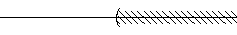
\includegraphics{images/dedekind-schnitt}
  \caption{Ein Dedekindscher Schnitt}%
  \label{fig:schnitt}
\end{figure}

\begin{example}
  Sei $x = p/q \in \mathbb Q$. Setze $D_{x} = \left\{y \in \mathbb Q \mid y > x\right\}
  \subset \mathbb Q$.
  Dann ist $D_{x}$ ein Schnitt. Wir nennen $D_{x}$ einen \emph{rationalen Schnitt},
  da diese später die rationalen Zahlen in $\mathbb R$ werden.
\end{example}

\begin{remark}
  Seien $D, D' \subset \mathbb Q$ zwei Schnitte mit $D \neq D'$.
  Dann existiert $x \in \mathbb Q$ mit entweder $x \in D$ und $x \notin D'$,
  oder $x \notin D$ und $x \in D'$.
  Im ersten Fall gilt $D' \subset D$, und im zweiten Fall gilt $D \subset D'$.
\end{remark}

\begin{question}
  Sei $D \subset \mathbb Q$ ein Schnitt. Existiert
  eine Zahl $x \in \mathbb Q$ mit $D = D_{x}$?
  (Hier ist $D_{x}$ die Menge aus dem Beispiel oben.)
\end{question}

Wie erwartet ist die Antwort nein, siehe Proposition~\ref{prop:real-uncountable} unten.

\begin{definition}
  Die Menge $\mathbb R$ der \emph{reellen Zahlen} ist definiert als die Menge
  aller Dedekindscher Schnitte $D \subset \mathbb Q$.
\end{definition}

\begin{examples}
  \leavevmode
  \begin{itemize}
    \item Sei $p/q \in \mathbb Q$. Dann ist
      \[ D_{p/q} = \left\{x \in \mathbb Q \mid x> p/q \right\}\]
      ein rationaler Schnitt. So erhalten wir eine ``Einbettung''
      $\mathbb Q \to \mathbb R$.
    \item Nicht alle Schnitte sind rational. Zum Beispiel ist
      \[D_{\sqrt 2} = \left\{x \in \mathbb Q \mid x^{2} > 2 \text{ oder } x < 0\right\}\]
      kein rationaler Schnitt.
  \end{itemize}
\end{examples}

\begin{proposition}[Cantor]\label{prop:real-uncountable}
  Die Menge $\mathbb R$ ist überabzählbar, das heisst unendlich
  aber nicht abzählbar.
\end{proposition}

\begin{corollary}
  Es gibt irrationale Schnitte, das heisst Schnitte $D \subset \mathbb Q$,
  welche nicht vom Typ $D_{x}$ für $x \in \mathbb Q$ sind.
\end{corollary}

\begin{proof}
  Die Menge $\mathbb Q$ ist abzählbar (siehe Proposition~\ref{prop:q-countable}).
\end{proof}

\begin{proof}[Beweis von Proposition~\ref{prop:real-uncountable}]
  Wir erinnern uns an Proposition~\ref{prop:cantor} und ihr Korollar,
  die sagten, dass die Potenzmenge $P(\mathbb N )$ überabzählbar ist.
  Wir konstruieren nun eine injektive Abbildung
  $\psi \colon P(\mathbb N) \to \mathbb R$.
  Daraus folgt dann, dass $\mathbb R$ überabzählbar ist.

  Die Konstruktion von $\psi$ ist folgendermassen.
  Sei $B \in P(\mathbb N)$, das heisst $B \subset \mathbb N$.
  Schreibe $B = \{n_{0}, n_{1}, n_{2}, \dots\}$ mit $n_{0} < n_{1} < n_{2} < \dots$.
  Diese Menge könnte auch endlich sein.
  Definiere einen Schnitt
  \[
    D_{B} = \left\{x \in \mathbb Q \middle| x > \sum_{k=0}^{\infty}
      {\left( \frac{1}{3}\right)}^{n_{k}}
    \right\}.
  \]
  Es gilt zum Beispiel:
  \begin{enumerate}[(1)]
    \item Sei $B = \emptyset$.
      Wir halten uns an die Konvention ``leere Summe gleich $0$''. Es gilt also
      $D_{\emptyset} = D_{0}$.
    \item Sei $B = \mathbb N$, das heisst $B = \{0, 1, 2, \dots\}$
      (also $n_{k} = k$). Berechne
      \begin{align*}
        \sum_{k=0}^{\infty}
        {\left(\frac{1}{3}\right)}^{k}
        &= 1 + \frac{1}{3} + {\left(\frac{1}{3}\right)}^{2} + \dots \\
        &= \frac{1}{1 - 1/3}
          \\ &= \frac{3}{2}.
      \end{align*}
      Also ist $D_{\mathbb N} = D_{3/2}$.
  \end{enumerate}

Sei nun $B = \{n_{0}, n_{1}, \dots \} \subset \mathbb N$ beliebig.
Dann gilt
\begin{align*}
  0
  &\leq \sum_{k=0}^{\infty}{\left(\frac{1}{3}\right)}^{n_{k}} \\
  &\leq \sum_{k=0}^{\infty} {\left(\frac{1}{3}\right)}^{k} \\
  &= \frac{3}{2}.
\end{align*}
Also gilt $D_{0} \supset D_{B} \supset D_{3/2}$.
Insbesondere ist $D_{B} \neq \emptyset$ und $D_{B} \neq \mathbb Q$, das heisst
$D_{B}$ ist wirklich ein Schnitt.
Setze nun
\[\psi(B) = D_{B} \in \mathbb R.\]

Wir behaupten nun, das $\psi$ injektiv ist. Konkreter, seien
$B_{1}, B_{2} \in P(\mathbb N)$ mit $B_{1} \neq B_{2}$.
Wir zeigen, dass $D_{B_{1}} \neq D_{B_{2}}$.
Schreibe dazu
\begin{align*}
  B_{1} &= \{m_{0}, m_{1}, m_{2}, \dots\} \;\text{mit}\; m_{0} < m_{1} < m_{2} < \dots, \\
  B_{2} &= \{n_{0}, n_{1}, n_{2}, \dots\} \;\text{mit}\; n_{0} < n_{1} < n_{2} < \dots.
\end{align*}
Sei $\ell \in \mathbb N$ minimal mit $m_{\ell} \neq n_{\ell}$. So ein $\ell$
existiert, da $B_{1} \neq B_{2}$. Wir nehmen an, dass $m_{\ell} < n_{\ell}$.
Beispielsweise, für $B_{1} = \{0, 1, 2\}$ und $B_{2} = \{0, 1, 3, 4, 5\}$ ist
$\ell = 2$, $m_{2} = 2$ und $n_{2} = 3$.
Vergleiche die Summen
\begin{align*}
  S_{1} &= \sum_{k=0}^{\infty} {\left(\frac{1}{3}\right)}^{m_{k}}
          \geq \sum_{k=0}^{\ell} {\left(\frac{1}{3}\right)}^{m_{k}}
          = \sum_{k=0}^{\ell-1} {\left(\frac{1}{3}\right)}^{m_{k}} + {\left(\frac{1}{3}\right)}^{m_{\ell}}, \\
  S_{2} &= \sum_{k=0}^{\infty}{\left(\frac{1}{3}\right)}^{n_{k}}
          = \sum_{k=0}^{\ell - 1} {\left(\frac{1}{3}\right)}^{n_{k}}
          + \sum_{k= \ell}^{\infty} {\left(\frac{1}{3}\right)}^{n_{k}}.
\end{align*}
Setzen wir
\begin{align*}
  X &= \sum_{k=0}^{\ell - 1}{\left(\frac{1}{3}\right)}^{n_{k}}, \\
  Y &= \sum_{k= \ell}^{\infty} {\left(\frac{1}{3}\right)}^{n_{k}},
\end{align*}
so erhalten wir aus $n_{\ell} > m_{\ell}$, dass $n_{\ell} \geq m_{\ell} + 1$.
Also folgt
\[Y \leq {\left(\frac{1}{3}\right)}^{m_{\ell}} \cdot \left(
    \frac{1}{3} + {\left( \frac{1}{3}\right)}^{2} + \dots
    \right).\]
Es gilt also
\begin{align*}
  S_{1} & \geq X + {\left(\frac{1}{3}\right)}^{m_{\ell}}, \\
  S_{2} & \leq X + {\left(\frac{1}{3}\right)}^{m_{\ell}}\cdot \frac{1}{2}.
\end{align*}
Setze
\[x = X + \frac{2}{3}\cdot {\left(\frac{1}{3}\right)}^{m_{\ell}} \in \mathbb Q.\]
Dann ist $x < S_{1}$, also $x \notin D_{B_{1}}$, und $x > S_{2}$, also
$x \in D_{B_{2}}$. Wir schliessen, dass $\psi(B_{1}) \neq \psi(B_{2})$.
Also ist $\psi$ injektiv und $\mathbb R$ überabzählbar.
\end{proof}

\begin{question}
  Wo kommen all diese Schnitte $D_{B}$ her?
\end{question}

Es muss irrationale Schnitte $D_{B}$ geben (sonst wären es abzählbar viele).
Insbesondere muss es Teilmengen $B \subset \mathbb N$ geben, so dass die
entsprechende Summe
\[x = \sum_{k=0}^{\infty} {\left(\frac{1}{3}\right)}^{n_{k}}\]
keine rationale Zahl ist.
Die Menge all dieser Summen heisst \emph{Cantormenge}.

\subsection*{Eine Ordnung auf den reellen Zahlen}
Seien $D, D' \in \mathbb R$ mit $D \neq D'$. Dann gilt entweder
$D \subset D'$ oder $D' \subset D$ (siehe oben).
\begin{definition}
  Wir schreiben $D < D'$ falls $D' \subset D$ und $D' \neq D$.
\end{definition}

\begin{remark}
  Falls $D < D'$ (das heisst $D' \subset D$ und $D' \neq D$), dann
  existiert $y \in \mathbb Q$ mit $y \in D$ und $y \notin D'$.
  Da $D$ kein kleinstes Element enthält,
  existiert $x \in \mathbb Q$ mit $x < y$ und $x \in D$.
  Dann gilt $D' \subset D_{x} \subset D$, und all diese
  Inklusionen sind strikt. Die erste Inklusion ist strikt,
  da $x < y$. Das war nötig, da $D' = D_{y}$
  gelten könnte. Wir haben also eine rationale Zahl
  $x \in \mathbb Q$ gefunden mit
  $D < D_{x} < D'$.
  Wir haben somit gezeigt, dass zwischen zwei verschiedenen reellen
  Zahlen immer eine rationale Zahl liegt.
  Dies ist überraschend, da die Menge $\mathbb Q$
  abzählbar ist, aber nicht die Menge $\mathbb R$.

  Kronecker hat aus diesem Grund Dedekinds Arbeit nicht akzeptiert,
  und Poincaré hat es sogar als Teufelswerk bezeichnet.
  Aus diesem Skeptizismus ist unter anderem der
  Konstruktivismus in der Logik entstanden.
  Dieser hat jedoch nicht mehr viele Vertreter.
\end{remark}

\subsection*{Addition auf den reellen Zahlen}

\begin{definition}
Seien $D, D' \in \mathbb R$ Dedekindsche Schnitte.
Wir Definieren die \emph{Summe} von $D$ und $D'$ als
\[D + D' = \left\{z \in \mathbb Q \mid \text{ es existieren }
    x \in D \text{ und } y \in D' \text{ mit } z = x + y\right\}.\]
\end{definition}

Man kann leicht überprüfen, dass $D + D'$ ein Schnitt ist.

\begin{lemma}\label{lem:r-plus-gruppe}
  $\mathbb R$ mit Addition ist eine kommutative Gruppe mit neutralem Element
  \[D_{0} = \left\{x \in \mathbb Q \mid x > 0\right\}\]
\end{lemma}

\begin{proof}
  \leavevmode
  \begin{itemize}
    \item Kommutativität und Assoziativität übertragen sich von der Addition
      auf $\mathbb Q$.
    \item $D_{0}$ ist das neutrale Element. Zu prüfen ist
      für alle $D \in \mathbb R$, dass $D + D_{0} = D$. Wir
      zeigen beide Inklusionen.
      \begin{enumerate}[(a)]
        \item Die Inklusion $D + D_{0} \subset D$ folgt direcht aus
          der Definition: Wenn wir eine positive Zahl
          (ein Element von $D_{0}$) zu einem
          $x \in D$ addieren, erhalten wir eine grössere
          rationale Zahl als $x$, die dementsprechend auch in $D$ ist.
        \item Die umgekehrte Inklusion $D + D_{0} \supset D$ zeigen
          wir wie folgt. Sei $y \in D$. Dann existiert $x \in D$ mit
          $x < y$, da $x$ nicht das kleinste Element von $D$ ist.
          Dann gilt $y = x + (y - x) \in D + D_{0}$, da $x \in D$
          und $0 < y - x \in D_{0}$.
      \end{enumerate}
      Aus (a) und (b) folgt $D = D + D_{0}$, also ist $D_{0}$ das
      neutrale Element von $\mathbb R$.
    \item Die inversen Elemente müssen wir erst noch konstruieren.
      Das ist der womöglich schwierigste Schritt in diesem Beweis.
      Wir definieren
      \[-D = -(\mathbb Q \setminus D) + D_{0},\]
      Das ist scheinbar die einfachste Art, dies aufzuschreiben.
      Für ein wenig Inutition dahinter, siehe
      Abbildung~\ref{fig:additiv-dedekind}.
      Hier ist zu beachten, dass das Minus auf der linken Seite
      anders zu interpretieren ist, als das Minus auf der rechten
      Seite.
      Wir behaupten nun, dass $D + (-D) = D_{0}$. Berechne dazu
        \[D + (-D) = D  + (-(\mathbb Q \setminus D)) + D_{0}.\]
      Seien $x \in D$, $y \in -(\mathbb Q \setminus D)$, und $z \in D_{0}$.
      Dann gilt:
      \begin{enumerate}[(i)]
        \item $z > 0$,
        \item $-y \in \mathbb Q \setminus D$, also $y \notin D$.
          Das heisst $-y < x$, also $x + y > 0$.
      \end{enumerate}
      Wir schliessen, dass $x + y + z > 0$, also $x + y + z \in D_{0}$.
      Das zeigt die Inklusion $D + (-D) \subset D_{0}$. 
      
      Sei umgekehrt
      $p/q \in D_{0}$, das heisst $p/q > 0$. Wähle $y \in \mathbb Q$
      mit $0 < y < p/q$, zum Beispiel $y = p/2q$.
      Es existiert $x \in D$, so dass $x - y \notin D$:
      Sei hierzu $x' \in D$ beliebig, und sei $n \in \mathbb N$ maximal
      so dass $x' -ny \in D$. Dann erfüllt $x = x' - ny$ diese Eigenschaft.
      Aus $x - y \notin D$ folgt, dass $x- y \in \mathbb Q \setminus D$.
      Dann ist aber $y - x \in - (\mathbb Q \setminus D)$.
      Also ist $p/q = x + (y-x) + (p/q - y)$, wobei
      $x \in D$, $y - x \in -(\mathbb Q \setminus D)$, und $p/q - y \in D_{0}$.
      Also liegt $p/q$ in $D + (-D) = D + (-(\mathbb Q \setminus D)) + D_{0}$,
      also $D + (-D) \supset D_{0}$. Wir haben beide Inklusionen gezeigt,
      und somit
      erhalten wir $D + (-D) = D_{0}$. \qedhere
  \end{itemize}
\end{proof}

\begin{figure}[htb]
  \centering
  \begin{minipage}{0.4\linewidth}
    \centering
    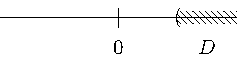
\includegraphics{images/dedekind-additiv-invers1}
  \end{minipage}%
  \begin{minipage}{0.4\linewidth}
    \centering
    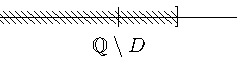
\includegraphics{images/dedekind-additiv-invers2}
  \end{minipage}
  \begin{minipage}{0.4\linewidth}
    \centering
    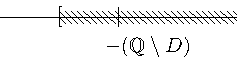
\includegraphics{images/dedekind-additiv-invers3}
  \end{minipage}%
  \begin{minipage}{0.4\linewidth}
    \centering
    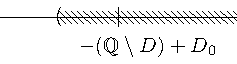
\includegraphics{images/dedekind-additiv-invers4}
  \end{minipage}
  \caption{Additive Inverse}%
  \label{fig:additiv-dedekind}
\end{figure}

\subsection*{Multiplikation auf den reellen Zahlen}
Dieser Abschnitt verläuft völlig analog zum letzten,
aber wir müssen mit den Vorzeichen vorsichtig sein.

\begin{definition}
Seien
$D ,D' \in \mathbb R$. Wir nehmen an, dass $D, D' \geq 0$,
das heisst $D, D' \subset D_{0}$. Dann definieren wir das \emph{Produkt}
von $D$ und $D'$ als
\[D \cdot D' = \{z \in \mathbb Q \mid \textup{ es existieren } x \in D,
  y \in D' \textup{ mit } z = x \cdot y\}.\]
Falls $D < 0$ und $D' \geq 0$, dann definieren wir
\[D \cdot D' = -(-D) \cdot D',\]
falls $D \geq 0$ und $D' < 0$, definieren wir ähnlich
\[D \cdot D' = -(D \cdot (-D')),\]
und falls $D < 0$ und $D' < 0$ definieren wir
\[D \cdot D' = (-D) \cdot (-D').\]
In dieser Definition bezeichnet ``$-D$'' das in obigem Abschnitt
definierte additive Inverse von $D$ (und nicht die gespiegelte Menge).
\end{definition}

\begin{lemma}\label{lem:r-mal-gruppe}
  Die Menge $\mathbb R \setminus \{D_{0}\}$ mit Multiplikation ist eine
  kommutative Gruppe mit neutralem Element
  \[D_{1} = \{x \in \mathbb Q \mid x > 1\}.\]
\end{lemma}

\begin{proof}
  \leavevmode
  \begin{itemize}
    \item Die Kommutativität und Assoziativität der Multiplikation
      übertragen sich von $\mathbb Q$ auf $\mathbb R$.
    \item Wir müssen zeigen, dass $D_{1}$ tatsächlich das neutrale
      Element von $\mathbb R$ ist.
      Sei $D \in \mathbb R$. Zu prüfen ist, dass $D \cdot D_{1} = D$.
      Wir prüfen dies für $D > 0$. Die anderen Fälle sind nicht
      schwieriger, da müssen wir einfach an den entsprechenden Stellen
      ein Minussymbol hinschreiben.
      Wir zeigen wieder beide Inklusionen.
      \begin{enumerate}[(a)]
        \item Die Inklusion $D \cdot D_{1} \subset D$ ist klar nach Definition.
        \item Sei umgekehrt $y \in D$. Wähle $x \in D$ mit $x < y$ und $x > 0$.
          Dann ist \[y = x \cdot \frac{y}{x} \in D \cdot D_{1}\] da $y/x > 1$.
      \end{enumerate}
      Also ist $D \cdot D_{1} = D$.
    \item
      Sei $D \in \mathbb R$ mit $D \neq D_{0}$.
      Wir konstruieren $D^{-1}$, das multiplikative Inverse von $D$.
      Wir nehmen auch hier der Einfachheit halber $D > 0$ an,
      auch hier, um uns nicht zu viele Gedanken über das Platzieren
      der Minussymbole zu machen. Setze
      \[D^{-1} = {(D_{0} \setminus D)}^{-1} \cdot D_{1}.\]
      Auch hier bedeutet das Symbol ${}^{-1}$ links etwas anderes als rechts.
      Für Intuition dazu betrachte Abbildung~\ref{fig:multiplikativ-dedekind}.
      Wir testen wieder beide Inklusionen.
      \begin{enumerate}[(a)]
        \item Für $x \in D$, $y \in {(D_{0} \setminus D)}^{-1}$, und
          $z \in D_{1}$ ist $x \cdot y \cdot z > 1$.
          Wir schliessen, dass $D \cdot D^{-1} \subset D_{1}$.
        \item Sei $p/q \in D_{1}$, das heisst $p/q > 1$.
          Wähle $y \in \mathbb Q$ mit $1 < y < p/q$, zum Beispiel
          \[y = \frac{p + q}{2q}.\]
          Wähle $x \in D$ mit $x/y \notin D$. Dann gilt:
          \[\frac{p}{q} = x \cdot \frac{y}{x} \cdot
            \frac{p/q}{y}\in D \cdot
          {(D_{0} \setminus D)}^{-1} \cdot D_{1}.\]
          Da $x/y \notin D$ ist $x / y \in D_{0} \setminus D$,
          also $y/x \in {(D_{0} \setminus D)}^{-1}$.
          Wir erhalten die umgekehrte Inklusion $D \cdot D^{-1} \supset D_{1}$.
      \end{enumerate}
      Setzen wir (a) und (b) zusammen, erhalten wir $D \cdot D^{-1} = D_{1}$.
      \qedhere
  \end{itemize}
\end{proof}

\begin{figure}[htb]
  \centering
  \begin{minipage}{0.4\linewidth}
    \centering
    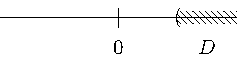
\includegraphics{images/dedekind-multiplikativ-invers1}
  \end{minipage}%
  \begin{minipage}{0.4\linewidth}
    \centering
    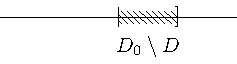
\includegraphics{images/dedekind-multiplikativ-invers2}
  \end{minipage}
  \begin{minipage}{0.4\linewidth}
    \centering
    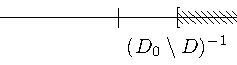
\includegraphics{images/dedekind-multiplikativ-invers3}
  \end{minipage}%
  \begin{minipage}{0.4\linewidth}
    \centering
    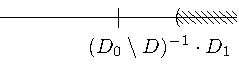
\includegraphics{images/dedekind-multiplikativ-invers4}
  \end{minipage}%
  \caption{Multiplikative Inverse}%
  \label{fig:multiplikativ-dedekind}
\end{figure}

\begin{exercise}
  Überprüfe, dass $D_{\sqrt 2} \cdot D_{\sqrt 2} = D_{2}$.
\end{exercise}

\begin{remark}[Zur Notation]
  Ab jetzt schreiben wir $p/q$ anstatt $D_{p/q}$,
  auch wenn wir $p/q$ als reelle Zahl (also als Schnitt)
  meinen.
  Ebenso schreiben wir $\sqrt 2$ statt $D_{\sqrt 2}$.
  Ausserdem benutzen wir Variablen $x,y,z, \dots$
  für reelle Zahlen.
  Das ist ein bisschen gefährlich, da wir immer noch
  Axiome zu überprüfen haben, bis wir unser Ziel zu Beginn
  des Abschnitts erreichen. Das sollte jedoch nicht allzu
  viele Missverständnisse bereiten.
\end{remark}

\subsection*{Eine Ordnung auf den reellen Zahlen (Reprise)}
\begin{definition}
  Seien $D, D' \in \mathbb R$. Wir schreiben $D \leq D'$ falls
  $D \supset D'$ und $D < D'$ falls $D \supset D'$ und $D \neq D'$.
\end{definition}

\begin{definition}
  Ein \emph{geordneter Körper} ist ein Körper $(K, +, \cdot)$
  zusammen mit einer binären Relation $\leq$, welche folgende
  Eigenschaften hat.
  \begin{enumerate}[(i)]
    \item Für alle $x, y \in K$ gilt $x \leq y$ oder $y \leq x$,
      und $x = y$ genau dann, wenn $x \leq y$ und $y \leq x$.
    \item Für alle $x, y, z \in K$ gilt, dass immer wenn
      $x \leq y$ und $y \leq z$, dann auch $x \leq z$. Diese
      Eigenschaft nennt man \emph{Transitivität}.
    \item Für alle $x, y, z \in K$ gilt, dass immer wenn
      $x \leq y$, dann auch $x + z \leq y + z$.
    \item Für alle $x, y, z \in K$ gilt, dass immer wenn
      $x \leq y$ und $0 \leq z$, dann auch $xz \leq yz$.
  \end{enumerate}
  Bei den Eigenschaften (iii) und (iv) spricht man von additiver,
  beziehungsweise multiplikativer \emph{Monotonie}.
\end{definition}

\begin{example}
  Die Menge der rationalen Zahlen $\mathbb Q$ mit der üblichen
  Addition, Multiplikation und Ordnung, ist ein geordneter Körper.
  Mit der ``üblichen Ordnung'' ist die Relation
  \[ \frac{a}{b} \leq \frac{c}{d} \Leftrightarrow ad \leq bc\]
  falls $b, d > 0$, gemeint.
  Wie die Ordnung auf $\mathbb Z$ zu verstehen ist, überlassen
  wir den Mengentheoretikern und fassen das als intuitiv genug auf.
\end{example}

\begin{theorem}
  Die Menge der reellen Zahlen $\mathbb R$ mit der oben definierten
  Addition, Multiplikation und Ordnung, ist ein geordneter Körper.
\end{theorem}

\begin{proof}
  \leavevmode
  \begin{itemize}
    \item Nach Lemma~\ref{lem:r-plus-gruppe} und 
      Lemma~\ref{lem:r-mal-gruppe} sind $(\mathbb R, +)$ und
      $(\mathbb R \setminus \{0\}, \cdot)$ kommutative Gruppen.
    \item Das Distributivgesetz überträgt sich von $\mathbb Q$
      auf $\mathbb R$.
    \item Die Ordnungsaxiome (i) bis (iv) sind leicht zu überprüfen.
      \qedhere
  \end{itemize}
\end{proof}

\subsection*{Vollständigkeit der reellen Zahlen}
Eine sehr wichtige Eigenschaft von $\mathbb{R}$, die
glücklicherweise direkt aus der Definition folgt,
ist die Vollständigkeit. Vage gesagt bedeutet das,
dass $\mathbb{R}$ keine ``Löcher'' hat.

\begin{definition}
	Sei $X$ 
	eine geordnete Menge. Dann heisst $X$ \emph{vollständig},
	falls für alle nichtleeren Teilmengen $A, B \subset X$
	mit $A < B$ (das heisst für alle $a \in A$ und alle $b \in B$
	gilt $a < b$) ein Element $c \in X$ mit $A \leq c \leq B$
	existiert.
\end{definition}

\begin{claim}
	Die Menge $\mathbb{R}$ der reellen Zahlen ist vollständig.
\end{claim}

\begin{proof}
  Setze
  \[
    D = \bigcup_{b \in B} D_b = \left\{x \in \mathbb{Q} \mid x > b
    \text{ für ein } b \in B \right\}.
  \]
  Diese Menge $D$ ist ein Schnitt (wieso?) %TODO
  \begin{itemize}
	  \item Es gilt für alle $b \in B$, dass $D \supset D_b$.
	  \item Es gilt für alle $a \in A$ und $b \in B$, dass
		  $D_a \supset D_b$.
  \end{itemize}
  Daraus folgt, dass 
	\[
	   D_a 
	   \supset 
	   \bigcup_{b \in B} D_b = D.
	\]
  Also repräsentiert der Schnitt $D$ eine reelle Zahl $c$
  mit den gewünschten Eigenschaften: für alle
  $D_a \in A$ und alle $D_b \in B$ existiert $D = D_c$
  mit $D_a \supset D_c \supset D_b$.
\end{proof}

\begin{remark}
  In $\mathbb Q$ liegt zwischen jedem Paar von rationalen Zahlen
  $a/b < c/d$ eine rationale Zahl, zum Beispiel die Zahl
  \[
    \frac{a+c}{b+d}.
  \]
  Das heisst aber nicht, dass $\mathbb Q$ vollständig ist:
  Tatsächlich ist $\mathbb{Q}$ nicht vollständig. Betrachte
  beispielsweise 
  $B= D_{\sqrt 2} = \left\{x \in \mathbb{Q} \mid x > \sqrt 2 \right\}$
  und $A = \mathbb{Q} \setminus D_{\sqrt 2}
  = \left\{x \in \mathbb{Q} \mid x < \sqrt 2\right\}$.
  Es existiert keine Zahl $c \in \mathbb{Q}$ mit $A \leq c \leq B$,
  da $\sqrt 2 \notin \mathbb{Q}$.
\end{remark}

\begin{einschub}
  Wie gut lässt sich $\sqrt 2$ durch rationale Zahlen
  approximieren? Es finden sich rationale Zahlen $p/q$ beliebig
  nahe an $\sqrt 2$ so dass
  \[
    \left\vert \sqrt 2 - \frac{p}{q} \right\vert < \frac{1}{q},
  \]
  sogar
  \[
    \left\vert \sqrt 2 - \frac{p}{q} \right\vert < \frac{1}{2q^2},
  \]
  aber nicht so, dass
  \[
    \left\vert \sqrt 2 - \frac{p}{q} \right\vert < \frac{1}{5q^2}.
  \]
  Man kann das mit \emph{Fordkreisen} veranschaulichen:
  Es ist nämlich nichts speziell an $\sqrt 2$. Jede reelle Zahl
  lässt sich so genau approximieren.
  % TODO Bild
\end{einschub}

\subsection*{Eindeutigkeit der reellen Zahlen}
\begin{theorem}[Dedekind]
  Seien $K_1$ und $K_2$ zwei vollständig geordnete Körper.
  Dann existiert ein Körperisomorphismus
  $\varphi\colon K_1 \to K_2$, das heisst
	   für alle $x, y \in K_1$ ist $\varphi(x+y)
		  = \varphi(x) + \varphi(y)$,
		  und $\varphi(xy) = \varphi(x)\varphi(y)$,
	und $\varphi$ ist bijektiv.
\end{theorem}
Wir beweisen dies in dieser Vorlesung nicht.
Man findet das in vielen Lehrbüchern der Analysis.
Um die Hauptidee des Beweises selber zu entdecken,
versuche zu zeigen, dass es nur einen Körperisomorphismus
$\mathbb{R} \to \mathbb{R}$ gibt.

Was dieses Theorem für uns bedeutet ist, dass wir ab jetzt
nur noch die Eigenschaften von $\mathbb{R}$, aber nicht
die Definition verwenden.

\subsection*{Folgerungen aus der Vollständigkeit}
\subsubsection*{Das Supremumsprinzip}
\begin{supremum}
Sei $A \subset \mathbb{R}$ nach oben beschränkt,
das heisst es existiert $b \in \mathbb{R}$ so dass
für alle $a \in A$ gilt, dass $a \leq b$.
Dann existiert eine eindeutige Zahl $S = \sup A$
mit folgenden Eigenschaften:
%TODO notation $A \leq B$ auslagern
\begin{enumerate}[\normalfont(i)]
	\item $A \leq S$ (das heisst $S$ ist eine obere Schranke
		für $A$). Präziser: für alle $a \in A$
		ist $a \leq S$.
  \item für alle $y \in \mathbb{R}$ mit $y < S$ gilt,
	  dass $A \not \leq y$ (das heisst $S$ ist die kleinste
	  obere Schranke für $A$). Präziser: für alle $y \in \mathbb{R}$
	  mit $y < S$ existiert $a \in A$ mit $y < a$.
\end{enumerate}
\end{supremum}

Die Zahl $\sup A$ heisst \emph{Supremum} von $A$. Falls
$\sup A \in A$, dann heisst diese Zahl auch \emph{Maximum} von $A$,
notiert $\max A$.

Analog sind die Begriffe \emph{Infimum} ($\inf A$) und
\emph{Minimum} ($\min A$) für nach unten beschränkte
Teilmengen von $\mathbb{R}$ definiert.
 
\begin{example}
  Sei $A = \left\{x \in \mathbb{R} \mid x < \sqrt 2\right\}$.
  Dann ist $\sup A = \sqrt 2$ kein Maximum, da $\sqrt 2 \notin A$.
  Hingegen für 
  $\bar A = \left\{x \in \mathbb{R} \mid x \leq \sqrt 2\right\}$
  ist $\sup \bar A = \sqrt 2$ ein Maximum.

  Die Menge $B = \left\{x \in \mathbb{Q} \mid x < \sqrt 2\right\}$
  hat aber kein Supremum in $\mathbb{Q}$, wenn wir das analoge
  Konzept in diesem 
  geordneten Körper definieren. 
\end{example}

\begin{proof}[Beweis der Existenz von $\sup A$]
  Definiere
  \[
	  B = \left\{x \in \mathbb{R} \mid \text{für alle } a \in A
  \text{ gilt } a < x\right\},
  \]
  die Menge aller oberen Schranken von $A$. Es gilt $A < B$
  nach der Definition von $B$.
  Nach Vollständigkeit existiert $c \in \mathbb{R}$
  mit $A \leq c \leq B$.
  Insbesondere ist $c$ eine obere Schranke für $A$.
  Wir nehmen nun widerspruchsweise an, es gäbe eine
  kleinere obere Schranke $y \in \mathbb{R}$ für $A$,
  das heisst $A \leq y < c \leq B$.
  Dann gilt
  \[
    A < \frac{y + c}{2} < B.
  \]
  Nach Definition der Menge $B$ wäre
  $(y + c)/2 \in B$, was im Widerspruch zu $(y +~c)/2~<~B$ steht.
  Die Zahl $\sup A = c$ hat also die gewünschten Eigenschaften.
\end{proof}

\subsubsection*{Das Archimedische Prinzip}
Das Archimedische Prinzip ist sehr intuitiv, war aber in
unserer Axiomatisierung nicht vertreten. Wir können
es aber aus der Vollständigkeit herleiten.

\begin{archimedes}[Archimedisches Prinzip]
  Sei $a \in \mathbb{R}$. Dann existiert eine natürliche
  Zahl $N \in \mathbb{N}$ mit $a < N$.
\end{archimedes}

\begin{proof}
  Sei $a \in \mathbb{R}$ fest. Setze
  \[
    A = \left\{n \in \mathbb{N} \mid n \leq a\right\} \subset \mathbb{N}
    \subset \mathbb{R}.
  \]
  Falls $A = \emptyset$, dann setze $N = 1$.
  Falls $A \neq \emptyset$, dann hat $A$ ein Supremum
  $S = \sup A \in \mathbb{R}$, da $A$ nach oben 
  durch $a$ beschränkt ist.
  Es ist dann $S - 1/2$ keine obere Schranke für $A$. 
  Also existiert eine Zahl $M \in A$ mit $M > S - 1/2$.
  Also ist $M + 1 > S$ und somit $N = M + 1 > a$. Diese Zahl ist
  natürlich, da $M$ als Element von $A$ eine natürliche Zahl ist.
\end{proof}
\end{document}
